\documentclass[10pt,a4paper]{article}
\input{AEDmacros}
\usepackage{etoolbox}
\usepackage{adjustbox}
\usepackage{inconsolata}
\usepackage{tcolorbox}
\usepackage{xcolor}
\usepackage{ragged2e}
\usepackage{changepage}
\usepackage{amssymb}
\usepackage[outputdir=out]{minted}
\DeclareRobustCommand{\ttfamily}{\fontencoding{T1}\fontfamily{lmtt}\selectfont}

\lstset{
  basicstyle=\ttfamily,
  numbers=none,
  frame=none,
  xleftmargin=10px,
  aboveskip=0pt
}
\newcommand{\vacio}{\emptyset}
\newcommand{\limn}{\lim_{n \to \infty}}
\newcommand{\ceil}[1]{%
  \left\lceil #1 \right\rceil%
}
\newcommand{\reales}{\mathbb{R}}
\newcommand{\limite}[2]{%
  \lim_{#1 \to #2}
}

\newenvironment{groupIzq}[1]{%
  \begin{list}{}{%
      \setlength{\leftmargin}{#1}%
      \setlength{\topsep}{0pt} % Elimina el espacio superior
      \setlength{\partopsep}{0pt} % Asegura que no haya espacio extra
    }
  \item[]
}{%
  \end{list}
}
\newcommand{\demoline}{\vspace{0.5em}}

\newcommand{\Indent}{\hspace*{0.75cm}}
\newcommand{\MiniIndent}{\hspace*{0.325cm}}
\newcommand{\Int}{\ensuremath{int}}

\newcommand{\Extends}[2]{%
  \noindent\ensuremath{\texttt{\textbf{#1}}\ \texttt{\textbf{extends}}\ #2}%
  \par
}
\newcommand{\Array}[1]{\ensuremath{Array \texttt{<}#1\texttt{>}}}
\newcommand{\Tupla}[1]{\ensuremath{Tupla \texttt{<}#1\texttt{>}}}
\newcommand{\Tuple}[1]{\ensuremath{Tuple \texttt{<}#1\texttt{>}}}
\newcommand{\Clase}[2]{\texttt{#1<#2>}}
\newcommand{\Type}[2]{%
  \noindent\ensuremath{\texttt{\textbf{#1}} = #2}%
  \par
}
\newcommand{\primitiva}[1]{\ensuremath{#1}}
\newcommand{\Arr}[1]{\ensuremath{Array \langle #1 \rangle}}
\newcommand{\conj}[1]{\ensuremath{conj \langle #1 \rangle}}
\newcommand{\union}{\cup}
\newcommand{\interseccion}{\cap}
\newcommand{\Struct}[1]{\ensuremath{\texttt{Struct} \langle \texttt{#1} \rangle}}
\newcommand{\StructField}[2]{\normalfont\ttfamily{#1}: \ensuremath{#2}}
\newcommand{\Title}[1]{%
  \raggedright
  \noindent{\textbf{#1}}%
  \justifying
  \vspace{1em}%
}

\newcommand{\TitlePar}[1]{%
  \raggedright
  \noindent{\textbf{#1}}%
  \justifying%
}

\newcommand{\Var}[2]{%
  \noindent\texttt{var \textbf{#1}}: #2 \par
}
\newenvironment{Vars}{%
  \begin{flushleft} % Alineación a la izquierda
}{%
  \end{flushleft}
  \vspace{1em} % Salto de línea final
}

\newenvironment{ModuloImplements}[2]{%
  \raggedright
  \texttt{Modulo #1\ implements\ #2\ \{}
  \justifying
  \begin{adjustwidth}{2em}{0em}
}{%
  \end{adjustwidth}
  \texttt{\}}%
}

\definecolor{lightgray}{gray}{1}
\definecolor{darkgray}{gray}{0.65}
\newcommand{\comentario}[1]{%
  \noindent{\normalfont\bfseries\ttfamily\small\textcolor{darkgray}{\% #1\ \ \%} \par}%
}

\newtcolorbox{ImplementationCodeBoxFixedWithParam}[1]{colback=lightgray!20, colframe=white, boxrule=0pt, left=5pt, right=5pt, top=5pt, bottom=5pt, width=#1}
\newtcolorbox{ImplementationCodeBoxFixed}{colback=lightgray!20, colframe=white, boxrule=0pt, left=5pt, right=5pt, top=5pt, bottom=5pt, width=0.8\linewidth}
\newtcolorbox{ImplementationCodeBox}{colback=lightgray!20, colframe=white, boxrule=0pt, left=5pt, right=5pt, top=5pt, bottom=5pt, width=\dimexpr\textwidth-2em\relax}
\definecolor{lightgray}{RGB}{220,220,220}
\newenvironment{ImplementationCode}[1]{%
  \VerbatimEnvironment
  \vspace{-0.2em}
  \begin{ImplementationCodeBoxFixedWithParam}{#1}
  \flushleft
  \begin{adjustbox}{minipage=\dimexpr\textwidth-2em\relax, margin=0pt}
  \begin{minted}[linenos, xleftmargin=-2.4em, numbersep=-2.5em]{java}%
}{
  \end{minted}
  \end{adjustbox}
  \vspace{-0.25em}
  \end{ImplementationCodeBoxFixedWithParam}
  \fussy
}

\usepackage{graphicx}
\usepackage{geometry}

\geometry{paperwidth=21cm, paperheight=80cm}

\begin{document}

\Title{Ejercicio 1}

\begin{figure}[h]
  \centering
  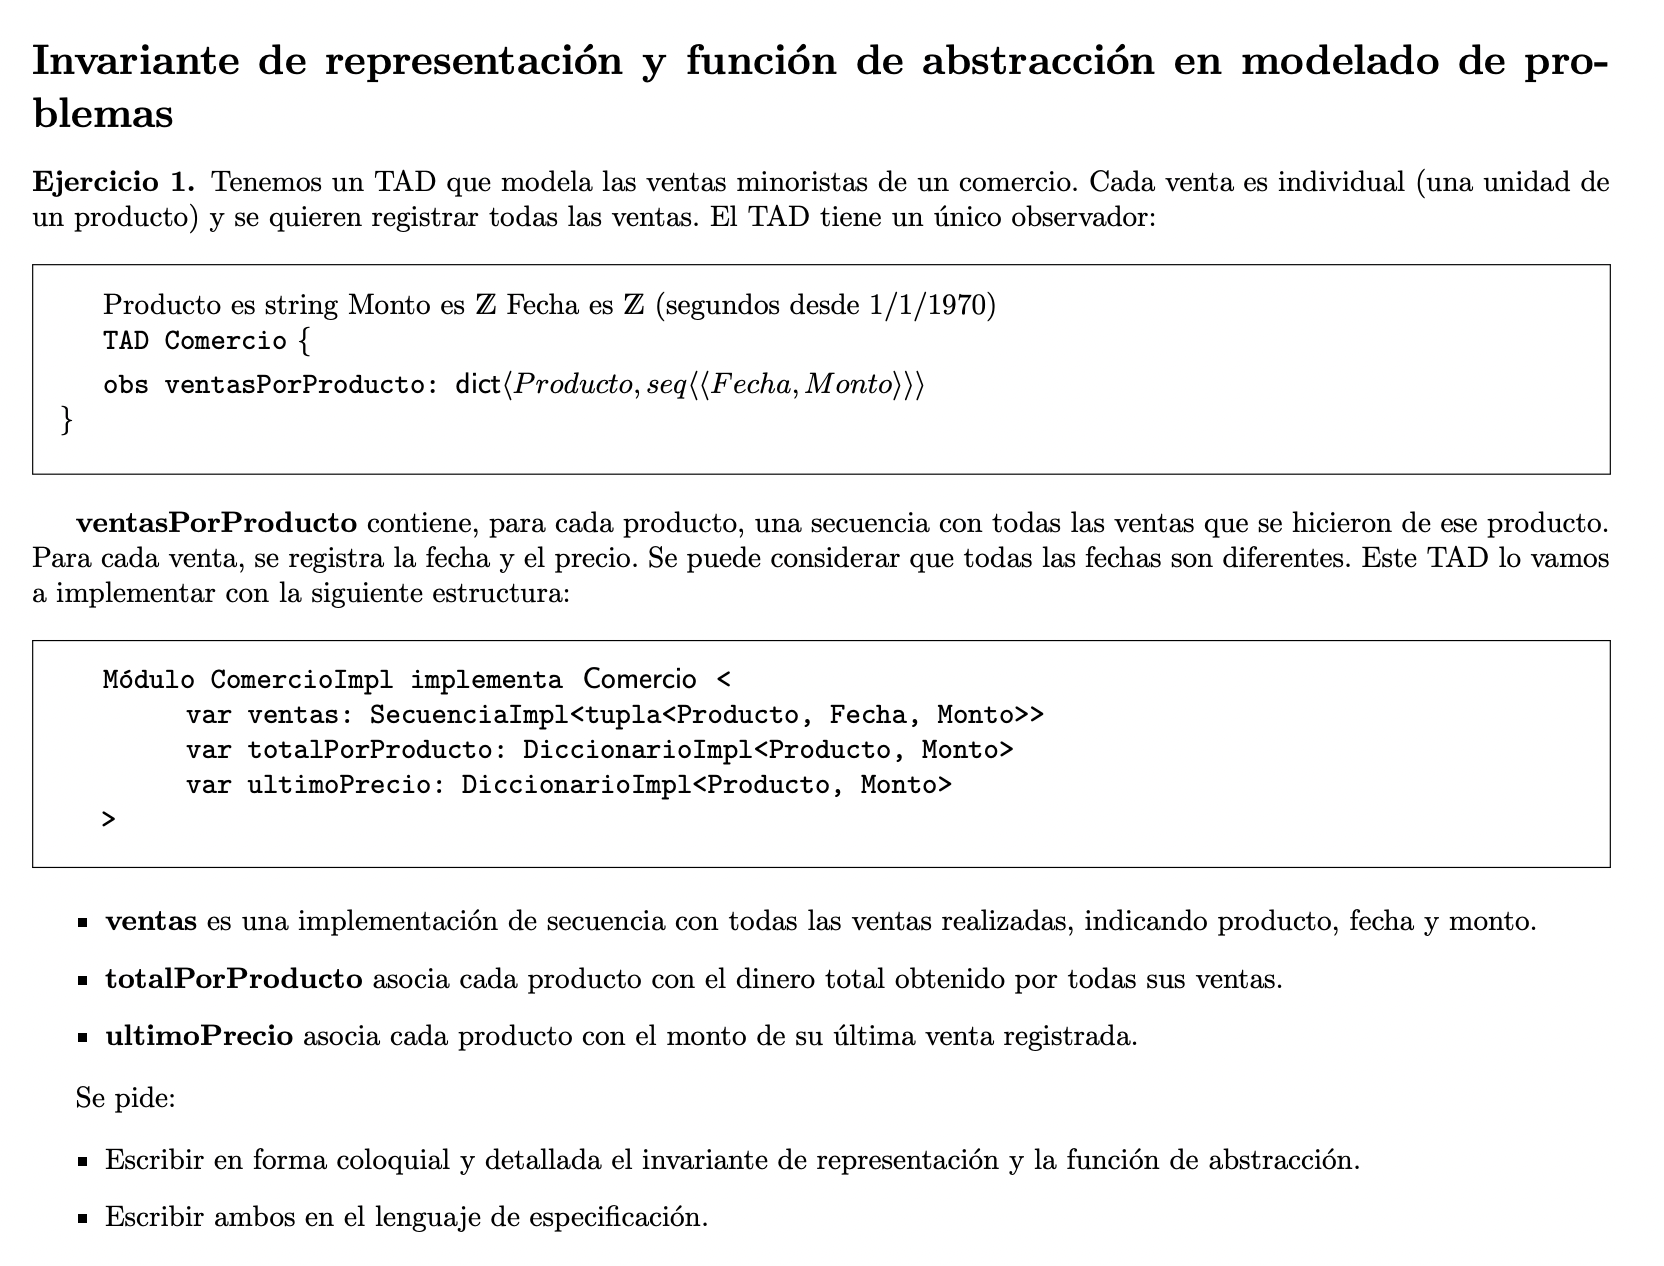
\includegraphics[width=\textwidth]{images/guia_8_ej_1.png}
  \caption{Enunciado Problema 1}
  \label{fig:ej_1}
\end{figure}

\vspace{1em}
\Type{Producto}{int}
\Type{Fecha}{int}
\Type{Monto}{float}
\Type{Ventas}{\Clase{SecuenciaImpl}{\Tupla{Producto, Fecha, Monto}}}
\vspace{1em}
\begin{ModuloImplements}{ComercioImpl}{Comercio}
  \begin{Vars}
    \Var{ventas}{Ventas}
    \Var{totalPorProducto}{\Clase{DiccionarioImpl}{Producto, Monto}}
    \Var{ultimoPrecio}{\Clase{DiccionarioImpl}{Producto, Monto}}
  \end{Vars}

  \aux{indiceDeFechaMasReciente}{c: ComercioImpl, $i_1$: \ent, $i_2$: \ent}{\ent}{
    IfThenElse(
      \\\Indent c.ventas.s[i_1]_1 > c.ventas.s[i_2]_1, i_1, i_2
    \\\hspace{0.65em})
  }
  \aux{indiceUltimoPrecio}{c: ComercioImpl, ventas: Ventas, inicio: \ent}{\ent}{
    IfThenElse(
      \\\Indent inicio = |ventas.s| - 1,
      \\\Indent inicio,
      \\\Indent indiceDeFechaMasReciente(c, inicio, ultimoPrecio(c, ventas, inicio + 1))
    \\\hspace{0.65em})
  }
  \aux{totalPorProducto}{c: ComercioImpl, producto: Producto}{\ent}{
    \\\Indent \displaystyle \sum_{i=0}^{|c.ventas.s|-1} IfThenElse(c.ventas.s[i]_0 = producto, c.ventas.s[i]_2, 0)
  }
  \vspace{1em}
  \pred{abs}{ab: \Clase{ArbolBinarioImpl}{T}, ab': \Clase{ArbolBinario}{T}}{
    Abs
  }
  \pred{invRep}{l: \Clase{ListaEnlazada}{T}}{
    InvRep
  }
\end{ModuloImplements}

\end{document}